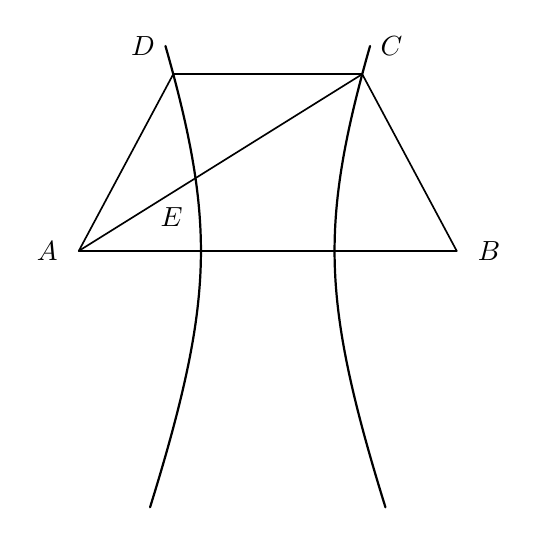
\begin{tikzpicture}[line width=0.6pt, line join=round, line cap=round, font=\normalsize]
  % trapezoid: A(-2.4,0) B(2.4,0) C(1.2,2.0) D(-1.2,2.0), |AB|=2|CD|
  \coordinate (A) at (-2.4,0);
  \coordinate (B) at (2.4,0);
  \coordinate (C) at (1.2000000000,2.2449944321);
  \coordinate (D) at (-1.2000000000,2.2449944321);
  % hyperbola x^2/a^2 - y^2/b^2 = 1, a=0.55, b=1.1, centered origin
  % right branch
  
  % left branch
  
  % trapezoid thin
  \draw (A) -- (B);
  \draw (B) -- (C);
  \draw (C) -- (D);
  \draw (D) -- (A);
  % diagonal A-C
  \draw (A) -- (C);
  \coordinate (E) at (-0.9176470588235295,0.9244094720265031);
% labels with clearance
  \node[left=4pt] at (A) {$A$};
  \node[right=4pt] at (B) {$B$};
  \node[above right=3pt] at (C) {$C$};
  \node[above left=3pt] at (D) {$D$};
  \node[below left=4pt,xshift=3pt,yshift=-3pt] at (E) {$E$};
\draw[line width=.8pt] plot[variable=\t,domain=-3.255241926493329:2.6041935411946633,samples=120] ({sqrt(0.72*(1+\t*\t/5.04))},\t);
\draw[line width=.8pt] plot[variable=\t,domain=-3.255241926493329:2.6041935411946633,samples=120] ({-sqrt(0.72*(1+\t*\t/5.04))},\t);
\end{tikzpicture}
